%%%%%%%%%%%% INTRODUCCIÓN  %%%%%%%%%%%%

\begin{center}
	{\fboxrule=4pt \fbox{\fboxrule=1pt
		\fbox{\LARGE{\bfseries 1. Introducción}}}} \\
	\addcontentsline{toc}{chapter}{1. Introducción}
	\setcounter{chapter}{1}
	\setcounter{section}{0}
	\rule{15cm}{0pt} \\
\end{center}

\pagenumbering{roman}
 
 \lettrine[lines=3, depth = 0]{E}{n} este documento explicar\'e c\'omo he llevado a cabo la práctica 2 de la asignatura \textbf{Sistemas Inteligentes} que consiste 
 en realizar un Sistema Basado en Reglas en un proceso de inferencia con encaminamiento hacia atrás con incertidumbre.
 \\siguiendo las especificaciones indicadas en el gui\'on del proyecto.
 
\section{Elementos de un SBR}
\par Los Sistemas Basados en Reglas (\texttt{SBR}) se inspiran en los sistemas de deducción en 
lógica proposicional o de primer orden. Constituyen un campo importante de la IA y 
a menudo se les llama \texttt{Sistemas Expertos (SE)} porque el conocimiento suele proceder de 
expertos humanos, y los \texttt{SBR} permiten capturarlo bien. Los \texttt{SBR}  constan de una base de 
conocimiento que contiene las reglas que definen el problema, una base de hechos que contiene los hechos 
establecidos como verdaderos tando de entrada como inferidos y un motor de inferencia encargado de ir 
obteniendo conclusiones tal y como indica la figura \ref{fig:SBR}.
 %%% IMAGEN DE SBR %%%
 \begin{figure}[H]
	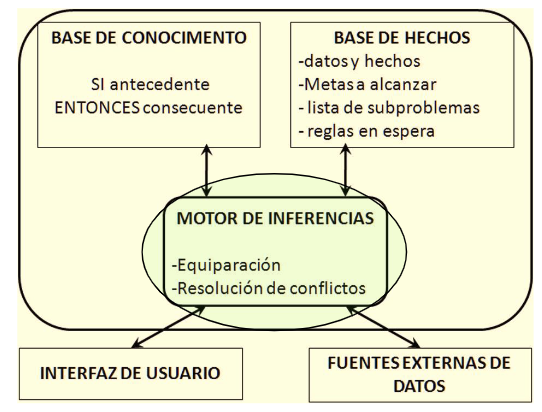
\includegraphics[width=\textwidth]{SBR}
	\centering
	\caption{Elementos de un Sistema Basado en Reglas.}
    	\label{fig:SBR}
\end{figure}


	\subsection{Base de Conocimiento (\texttt{BC})}
	\par Almacena porciones de conocimiento (estático) sobre cómo resolver el problema,
	cualquiera que sea la instancia de problema. Contiene las reglas que codifican todo el conocimiento. Defino una regla como un par condición-acción. 
	El antecedente contiene una lista de cláusulas a verificar y el consecuente una lista de acciones a ejecutar.

	\subsection{Base de Hechos (\texttt{BH})}
	\par Representa el estado actual de resolución de un problema concreto (dináminco). Contiene hechos establecidos como verdaderos, tanto datos de entrada como conclusiones inferidas.
	También se le llama \texttt{Memoria de Trabajo}.
	\par Contiene datos de entrada introducidos por el usuario o procedentes de sistemas externos tales como sensores o bases de datos. Además,
	esos datos de entrada pueden ser iniciales o introducidos durante el proceso, conforme el exterior proporciona
	nuevas evidencias. Contiene hechos inferidos por el sistema durante el proceso y las metas a alcanzar y sus subproblemas.
	\par Las reglas operan sobre el espacio de trabajo \texttt{BH} y es su único punto de unión entre ellas. La ejecución de una acción puede cambiar el contenido de la \texttt{BH}.

	\subsection{Mecanismo de Inferencias (\texttt{MI})}
	\par Es un mecanismo algorítmico. Selecciona las reglas que se pueden aplicar y las ejecuta, con el objetivo 
	de obtener alguna conclusión. Aplica la \texttt{BC} a los hechos conocidos almacenados en la \texttt{BH} y las conclusiones se 
	introducen, a su vez, en la \texttt{BH}. El objetivo se alcanza cuando este está contenido como hecho en la \texttt{BH}. 
	Si no es posible obtener un conjunto de reglas que permitan alcanzar dicho objetivo, la conclusión es que no hay solución porque es imposible llegar hasta él.
	Como se puede observar, la solución que obtiene un SBR está definida por un subconjunto de reglas que hacen cierto el hecho
	objetivo a partir de un subconjunto de hechos de entrada. Al \texttt{MI} también se le conoce como \texttt{Motor de Inferencias}.
	\par Existen dos formas de razonamiento:
	\begin{itemize}
		\item Encaminamiento hacia delante o \texttt{Dirigido por datos} es buscar el conjunto de metas que se verifican a partir de un conjunto de hechos.
	En este tipo de razonamiento, la inferencia progresa en la red de izquierda a derecha.
		\item Encaminamiento hacia atrás o \texttt{Dirigido por Metas} determina si se verifica una cierta meta con los hechos disponibles. Aquí,
	la inferencia progresa en la red de derecha a izquierda.
	\end{itemize}

\section{Representación mediante Factores de Certeza del conocimiento incierto}
	\par En muchos Sistemas Inteligentes es preciso considerar hechos cuya fiabilidad o precisión es limitada y
conocimiento en el que no tenemos una certeza absoluta. Es frecuente incorporar la incertidumbre sobre una
representación que originalmente no la incluye. 
	\par En una regla de un SBR, el factor de certeza es un coeficiente que es la credibilidad del consecuente o hipótesis en función de la 
	conjunción de antecedentes o evidencias. Los factores de certeza son valoraciones subjetivas proporcionadas por los expertos.
	\par Un factor de certeza se define en términos de dos componentes definidos subjetivamente:
	\begin{itemize}
		\item $MC(h,e)$: media de la creencia en la hipótesis \texttt{h}, dada la evidencia \texttt{e}. Es decir,
	\texttt{MC} mide hasta qué punto la evidencia soporta a la hipótesis.
		\item $MI(h,e)$: media de la incredulidad de la hipótesis \texttt{h}, dada la evidencia \texttt{e}. Es decir,
	\texttt{MI} mide hasta qué punto la evidencia soporta la negación de la hipótesis.
	\end{itemize}
	\par Una evidencia \texttt{e} no puede apoyar al mismo tiempo la creencia y la incredulidad en la hipótesis \texttt{h}. El factor de certeza 
	se define a partir de estos dos componentes, como $FC(h,e)=MC(h,e)-MI(h,e)$. Por tanto, \texttt{FC} 
	es un número entre -1 y 1. Normalmente basta con conocer uno de los tres valores, excepto cuando solo conocemos que $MI(h,e)=0$ ó $MC(h,e)=0$.
	\par \par La aplicación del razonamiento de los factores de certeza (\texttt{FC}) se realiza mediante encaminamiento hacia atrás que es un tipo de inferencia. Durante el 
	proceso de razonamiento, los \texttt{FCs} tienen que combinarse para reflejar el uso de las múltiples evidencias y reglas que se aplican. Las funciones de combinación de 
	factores de certeza se definen de la forma que satisfagan ciertas propiedades intuitivas, tal y como se muestra en la figura \ref{fig:factorCerteza}.
	 %%% IMAGEN DE SBR %%%
	 \begin{figure}[H]
		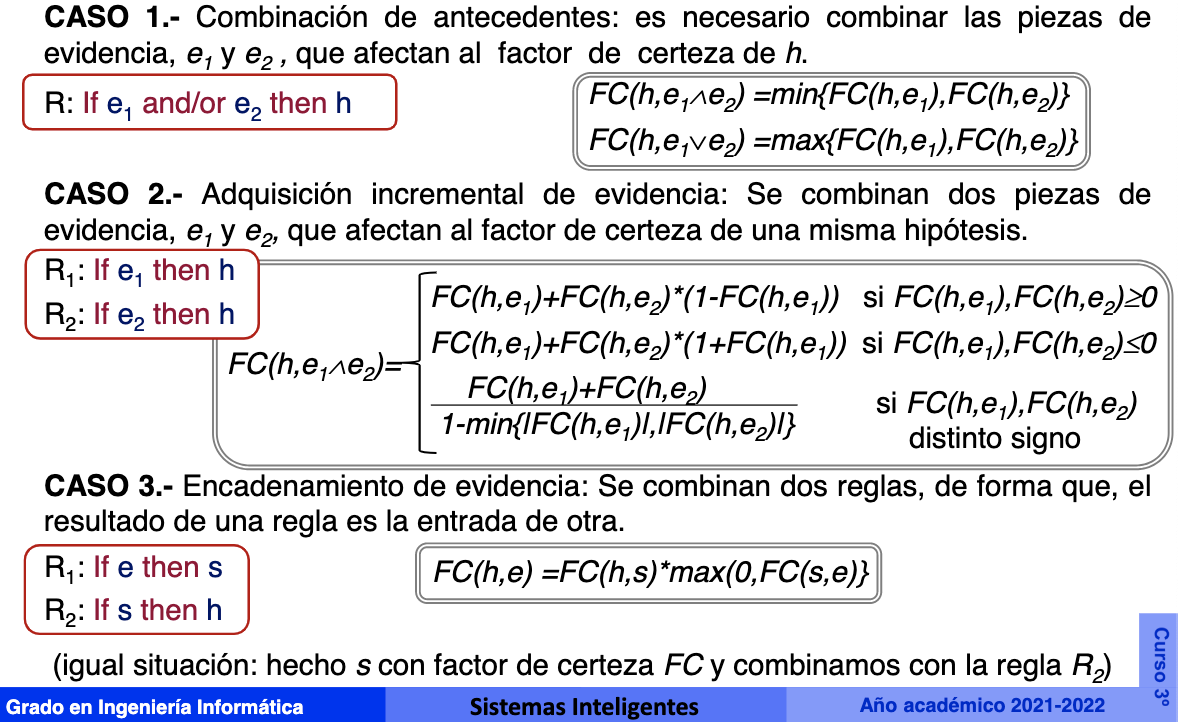
\includegraphics[width=\textwidth]{factoresCerteza}
		\centering
		\caption{Funciones de combinación de factores de certeza.}
			\label{fig:factorCerteza}
	\end{figure}
	\section{Cuestión}
\begin{ejer}
	1. ¿Qué es lo que mide un factor de certeza asociado a un hecho?
\end{ejer}
\par Solución: Mide la certeza de la evidencia de que ese hecho esté ocurriendo o sea cierto, es decir, mide la credibilidad del hecho.

\newpage
\pagenumbering{arabic}